\documentclass[a4paper, 11pt]{article}
\usepackage{comment} 
\usepackage{lipsum} %This package just generates Lorem Ipsum filler text. 
\usepackage{fullpage} % changes the margin
\usepackage[a4paper, total={7in, 10in}]{geometry}
\usepackage[fleqn]{amsmath}
\usepackage{amssymb,amsthm}  % assumes amsmath package installed
\newtheorem{theorem}{Theorem}
\newtheorem{corollary}{Corollary}
\usepackage{graphicx}
\usepackage{tikz}
\usetikzlibrary{arrows}
\usepackage{verbatim}
\usepackage[numbered]{mcode}
\usepackage{float}
\usepackage{tikz}
    \usetikzlibrary{shapes,arrows}
    \usetikzlibrary{arrows,calc,positioning}

    \tikzset{
        block/.style = {draw, rectangle,
            minimum height=1cm,
            minimum width=1.5cm},
        input/.style = {coordinate,node distance=1cm},
        output/.style = {coordinate,node distance=4cm},
        arrow/.style={draw, -latex,node distance=2cm},
        pinstyle/.style = {pin edge={latex-, black,node distance=2cm}},
        sum/.style = {draw, circle, node distance=1cm},
    }
\usepackage{xcolor}
\usepackage{mdframed}
\usepackage[shortlabels]{enumitem}
\usepackage{indentfirst}
\usepackage{hyperref}
\usepackage[capitalize, nameinlink]{cleveref}
\renewcommand{\thesubsection}{\thesection.\alph{subsection}}

\newenvironment{problem}[2][Problem]
    { \begin{mdframed}[backgroundcolor=gray!20] \textbf{#1 #2} \\}
    {  \end{mdframed}}

\newenvironment{reduction}
    { \begin{mdframed}[backgroundcolor=blue!20] \\}
    {  \end{mdframed}}
% Define solution environment

\newcommand{\hr}{\noindent\rule{7in}{2.8pt}}
\newenvironment{solution}
    {\textit{Solution:}}
    {\clearpage}
\newcommand{\prob}[1]{\begin{mdframed}[backgroundcolor=gray!20] \textbf{Problem #1}\end{mdframed}}
\renewcommand{\qed}{\quad\qedsymbol}
\newcommand{\bit}{\left\{0, 1\right\}}
\newcommand{\enc}{\mathsf{Enc}}
\newcommand{\dec}{\mathsf{Dec}}
\newcommand{\negl}{\mathsf{negl}}
\newcommand{\prf}{\mathsf{PRFAdv}}
\newcommand{\prg}{\mathsf{PRGAdv}}
\newcommand{\poly}{\mathsf{poly}}
\newcommand{\N}{\mathbb{N}}
\newcommand{\R}{\mathbb{R}}
\newcommand{\Z}{\mathbb{Z}}

\newcommand{\calA}{\mathcal{A}}
\newcommand{\calB}{\mathcal{B}}
\newcommand{\calC}{\mathcal{C}}
\newcommand{\calE}{\mathcal{E}}
\newcommand{\calF}{\mathcal{F}}
\newcommand{\calG}{\mathcal{G}}
\newcommand{\calH}{\mathcal{H}}
\newcommand{\calK}{\mathcal{K}}
\newcommand{\calM}{\mathcal{M}}
\newcommand{\calS}{\mathcal{S}}
\newcommand{\calX}{\mathcal{X}}
\newcommand{\calY}{\mathcal{Y}}

\newcommand{\inparen}[1]{\left{ #1 \right}}
\newcommand{\probtwo}[2]{\mathsf{Pr}_{#1}\left[ #2 \right]}
\newcommand{\set}[1]{\left\{ #1 \right\}}
\newcommand{\ct}{\mathsf{ct}}
\newcommand{\twotimessadv}[1]{\mathsf{2SSAdv}\left[ #1 \right]}



\newlength{\protowidth}
\newcommand{\pprotocol}[5]{
{\begin{figure*}[#3]
\begin{center}
\setlength{\protowidth}{\textwidth}
\addtolength{\protowidth}{-3\intextsep}

\fbox{
        \small
        \hbox{\quad
        \begin{minipage}{\protowidth}
    \begin{center}
    {\bf #1}
    \end{center}
        #5
        \end{minipage}
        \quad}

        }
        
\end{center}
\vspace{-4ex}
\caption{{#4} #2}
\end{figure*}
} }

% the first arg is name of security game
% the second arg is caption
% the third arg is the game description
% the label needs to be included 
\newcommand{\securitygame}[4]{
   \pprotocol{#1}{#2}{ht!}{#3}{#4}
}

\newcommand{\constr}[4]{
   \pprotocol{#1}{#2}{tbh!}{#3}{#4}
}

\begin{document}

\noindent
\large\textbf{Anish Banerjee, Shankh Gupta} \hfill \textbf{Problem Set - 1}   \\
\normalsize COL759: Cryptography \hfill August 2023\\
\hr


\prob{1: Perfect Two-time Security}
\begin{solution}
    \begin{enumerate}[(a)]
        \item Consider an Adversary $\calA$ that sends challenger the following pairs of messages : $(m_{00}, m_{01})$ and $(m_1, m_1)$. If $\calE$ were to be deterministic, the challenger would send either a pair of distinct ciphertexts (in case it encrypts the first pair, i.e. b = 0) or a pair of identical ciphtertexts (in case it encrypted the second pair, i.e. b = 1). In this scenario, $\calA$ would break the Encryption Scheme $\calE$ with certainity.
        
        But we can have randomized encryption schemes with randomness drawn from $\bit^{l_3}$. Still there is a non-zero probability of ${2^{-l_3}}$ of the two random strings selected to be same and thus the cipher texts will turn out to be same for two same messages. So the adversary performs the following : 
        
        \begin{itemize}
            \item The adversary sends two messages $(m_{00}, m_{01}), m_{00}\neq m_{01}$ and $(m_1, m_1)$ and receives ciphertext pair $(ct_0, ct_1)$ from the challenger.
            \item The adversary checks whether $ct_0 = ct_1$. If so, then $\calA$ guesses $b' = 1$ else it sends $b' = 0$.
        \end{itemize}
        Now, the advantage of $\calA$ will be:
        $$\mathsf{Adv}[\calA, \calG] =  \Big| \Pr[b'=1|b=0] - \Pr[b'=1|b=1] \Big| $$
        When b=0, the probability that two distinct messages get mapped to the same ciphertext using the same key is zero. Otherwise, we cannot decrypt it.
        $$\Pr[b'=1|b=0]=0$$
        On the other hand, when b=1, 
        $$\Pr[b'=1|b=1]\geq\Pr[b'=1|b=1, r_1=r_2]\Pr[r_1=r_2]=\frac{1}{2^{l_3}}$$ 
        where $r_1$ and $r_2$ are the random numbers used for the two encryptions. So the advantage is non-zero:
        $$\mathsf{Adv}[\calA,\calG] \geq 2^{-l_3}  $$
        And the winning probability is more than $1/2$:
        $$\Pr[\text{Adversary wins}]=\frac12+\frac12\mathsf{Adv}[\calA,\calG] \geq\frac{1}{2} + \frac{1}{2^{l_3 + 1}}$$
        Note that in the above derivation, we assumed that $r$ was sampled uniformly at random. Even if it were taken from some other distribution then too that probability will be non-zero.

        \item The encryption scheme $\calE = (\enc, \dec)$ which satisfies $ O(2^{-l}) $-perfect-two-time Security can be constructed as follows:
            $$\enc(k, m, r) = (r, m \oplus h_k(r))$$ and
            $$\dec(k, (ct_0, ct_1)) = ct_1 \oplus h_k(ct_0) $$
            where $r$ is a random string sampled from the Random space.
        To prove its security first consider the given PIF security game between a challenger $\calC$ and adversary $\calA$ (adversary can be inefficient):
        \begin{center}
            \textbf{PIF Security Game}
            \begin{itemize}
                \item The challenger samples uniformly a bit $b \gets \bit$ and a key $k \gets \calK$. 
                \item The adversary then sends two queries $x_0$ and $x_1$ to the challenger. If $b = 0$ then the challenger computes $h_k(x_0)$ and $h_k(x_1)$ and sends them to $\calA$. Else it samples uniformly a random function $f$ with input and output space as $\bit^{l} \rightarrow \bit^{l}$ and outputs $f(x_0)$ and $f(x_1)$.
                \item The adversary sends a bit $b'$ to the challenger.
            \end{itemize}
        \end{center}
        We claim that if $h_k$ is a Pairwise Independent Hash Function(PIF) then winning probability of $\calA$ in the above security game will be $\frac{1}{2}$. \\
        \textit{Proof} : We will prove the contrapositive. Suppose an adversary $\calA$ has non-zero advantage in the above PIF Game. $\calA$ performs the following : For every $k \in \calK$, it checks whether $h_k(x_0) = y_0 \And h_k(x_1) = y_1$ where $y_0$ and $y_1$ are the outputs sent by the challenger. If it finds such $k$, then $\calA$ sends $0$ to the challenger else it sends 1. \\ 
        Now $$\mathsf{PIFAdv}[\calA] = \Big| Pr[b'=0|b=0]-Pr[b'=0|b=1] \Big|$$ which is non-zero.
        Also $Pr[b'=0|b=0] = Pr[h_k(x_0) = y_0 \land h_k(x_1) = y_1]$
        and $Pr[b'=0|b=1]$ will be the same as getting two random strings of length l same as $h_k(x_0)$ and $h_k(x_1)$ which will be $\frac{1}{2^{2l}}$. So this implies that $Pr[h_k(x_0) = y_0 \land h_k(x_1) = y_1] \ne \frac{1}{2^{2l}}$ for some distinct $x_0$ and $x_1$ and $y_0$ and $y_1$. So this implies that $h_k$ is not a PIF.\\

        Now we need to prove that our construction which uses $\calH$ function family is almost perfect two time secure. We will prove the contra-positive that if there exists a ppt. adversary $\calA$ that breaks the security of our encryption scheme $\calE$ then the function family $\calH$ is not PIF, i.e., there exists a reduction algorithm $\calB$ that breaks the PIF security game. To prove this consider the following worlds: 
        \begin{itemize}
            \item \textbf{World-b} : Challenger encrypts message $m_b = (m_{b0}, m_{b1})$ and sends $ct = (ct_0, ct_1)$ to the adversary where $ct_0 = (r_0, Enc(k, m_{b0}, r_0))$ and $ct_1 = (r_1, Enc(k, m_{b1}, r_1))$. Let $p_b$ be the probability that $\calA$ outputs 0 in World-b.
            \item \textbf{Hybrid-World-b} : Challenger encrypts message  $m_b = (m_{b0}, m_{b1})$ by sampling a random function $f$ from the given input-output space and sends $ct = (ct_0, ct_1)$ to the adversary where $ct_0 = (r_0, m_{b0} \oplus f(r_0))$ and $ct_1 = (r_1, m_{b1} \oplus f(r_1))$. Let $p_{hyb,b}$ be the probability that $\calA$ outputs 0 in Hybrid-World-b.
        \end{itemize}

        Now given that $|p_0 - p_1|$ is non negligible, we can say that either $|p_0 - p_{hyb,0}|$ or $|p_1 - p_{hyb,1}|$ is non-negligible. Note that $p_{hyb,0}$ and $ p_{hyb,1}$ are only negligibly far apart (because of part(a)).

        \textbf{Observation} : There exists a reduction algorithm $\calB_i$ such that PIFAdv[$\calB$] = $|p_i - p_{hyb,i}|$. (where i = 0 or 1) \\
        \textit{Proof} : The algorithm $\calB_i$ samples two random strings $r_0$ and $r_1$ and sends them to the PIF challenger. It receives $m_0$ and $m_1$ from A and $f(r_0)$ and $f(r_1)$ from challenger. Now it sends $m_{i0} \oplus f(r_0)$ and $m_{i1} \oplus f(r_1)$. If f is a PIF function, then that corresponds to World-i for $\calA$ else it corresponds to Hybrid-World-i. So we can thereby say that the advantage of $\calB$ = $|p_i - p_{hyb,i}|$. (because $Pr[b'=0|b=0]$ is same as Pr[$\calA$ sends 0 in World-i] = $p_i$ and $Pr[b'=0|b=1]$ is same as Pr[$\calA$ sends 0 in Hybrid-World-i] = $p_{hyb,i}$).
        
    \end{enumerate}
\end{solution}


\prob{2 : Secure/Insecure PRGs and PRFs}
\begin{solution}
    \begin{enumerate}[(a)]
        \item PRGs
              \begin{enumerate}[i.]
                  \item $\calG' = \set{G'_n : \bit^{2n} \to \bit^{3n}}_{n \in \N}$, where $$ G'_n(s_1 ~||~ s_2) = G_n(s_1) \wedge G_n(s_2).$$
                        The given PRG is \textbf{insecure}. Consider the PRG game between $\calA$ and $G'$ challenger where on input $y$, $\calA$ outputs the last bit of $y$. Let $L(x)$ denote the last bit of $x$. Note that if $G$ is secure, then $\Pr[L(G(s))=0]$ will be close to 1/2. Otherwise, if it is $1/2+\epsilon$, we can create an adversary breaking $G$ with non-negligible advantage $\epsilon$ ($\calA$ always outputs 0). So, if we take $\Pr[L(G(s))=0]=1/2+\negl(\lambda)$
                        $$\Pr[b'=0|b=0]=\Pr[L(G(s_1)\wedge G(s_2))=0]$$
                        $$\leq\Pr[L(G(s_1))=0\wedge L(G(s_2))=0]+\Pr[L(G(s_1))=1\wedge L(G(s_2))=0]+\Pr[L(G(s_1))=0\wedge L(G(s_2))=1]$$
                        $$\approx3/4+\negl(\lambda)$$
                        and
                        $$\Pr[b'=0|b=1]=1/2$$
                        Thus the $\prg[\calA,\calG]\approx1/4$ which is non-negligible.

                  \item $\calG' = \set{G'_n : \bit^{2n} \to \bit^{3n}}_{n \in \N}$, where $$ G'_n(s_1 ~||~ s_2) = G_n(s_1) \oplus G_n(s_2)$$
                        This is a \textbf{secure} PRG. We prove the security by a hybrid argument.
                        \begin{itemize}
                            \item\textbf{World0} The challenger sends $G_n(s_1) \oplus G_n(s_2)$ to the attacker

                            \item\textbf{HybridWorld} The challenger sends $G_n(s_1) \oplus \mathsf{random}_1$ to the attacker

                            \item\textbf{World1} The challenger sends $\mathsf{random}_1\oplus\mathsf{random}_2$ to the attacker

                        \end{itemize}
                        \paragraph{Claim:} If any adversary $\calA$ can distinguish between World0 and HybridWorld then we can construct $\calB$ which breaks the PRG security of $G$. 

                        The reduction $\calB$ receives $y$ from the PRG challenger. It samples $s\gets\bit^n$ and sends $G(s)\oplus y$ to $\calA$. The advantage of $\calA$ in distinguishing between World0 and HybridWorld will be equal to the advantage of $\calB$ in breaking PRG security of $G$. 
                        
                        Similarly we can also claim that:

                        \paragraph{Claim:} If any adversary $\calA$ can distinguish between HybridWorld and World1 then we can construct $\calB$ which breaks the PRG security of $G$.

                        The reduction $\calB$ receives $y$ from the PRG challenger. It samples $r\gets\bit^n$ and sends $r\oplus y$ to $\calA$. The advantage of $\calA$ in distinguishing between HybridWorld and World1 will be equal to the advantage of $\calB$ in breaking PRG security of $G$.

                        Now we can choose any reduction randomly to break the PRG security of $G$. Also note that we cannot use a similar argument in part i. because $\mathsf{random}_1\wedge\mathsf{random}_2$ is not uniformly random.

              \end{enumerate}
        \clearpage
        \item PRFs
              \begin{enumerate}[i.]
                  \item $\calF' = \set{F'_n:\bit^{n} \times \bit^{2n} \to \bit^{n}}_{n\in \N}$ where $$F'_n(k, (x_1, x_2)) = F_n(k, x_1) \oplus F_n(k, x_2).$$

                        The given family $\calF'$ is \textbf{insecure}. Consider a PPT attacker $\calA$ who sends $\poly(\lambda)$ distinct $(x_i,x_i)$ queries to the  challenger. If the challenger chooses $b=0$ then it will end up sending $$F_n(k, x_i) \oplus F_n(k, x_i)=0^n$$ for each of the queries. The attacker outputs 0 if all the responses are 0 and 1 otherwise. Advantage of the attacker is close to 1, precisely $1-2^{-n\poly(\lambda)}$.

                  \item $\calF' = \set{F'_n:\bit^{n} \times \bit^{n} \to \bit^{n}}_{n\in \N}$ where $$F'_n(k, x) = F_n(k, x) \oplus x.$$

                        The given family is \textbf{secure}. Given an adversary $\calA$ which breaks PRF security of $\calF'$, we can construct an adversary $\calB$ which breaks the security of $\calF$ (\cref{red:p2bii})

                        \securitygame{Problem 2(b)(ii)}{Reduction for Problem 2(b)(ii)}{\label{red:p2bii}}
                        {
                            \begin{itemize}
                                \item Challenger picks a uniformly random bit $b \gets \bit$ and a seed $s\gets \bit^n$.
                                \item The adversary $\calA$ makes polynomially many queries to $\calB$, who passes them to the challenger. Challenger replies as in the PRF Game.
                                \item Upon receiving the response $y_i$ of each query, $\calB$ sends $ y_i\oplus x_i$ to $\calA$
                                \item After polynomially many queries, $\calB$ forwards the response send by $\calA$ $(b')$ and wins if $b=b'$.
                            \end{itemize}
                        }

                        It is clear from the reduction that the PRF advantage ($F$) of $\calB$ in the above game is same as the PRF advantage ($F'$) of $\calA$

              \end{enumerate}
    \end{enumerate}

\end{solution}

\prob{3 : PRG Security does not imply Related-Key-PRG Security}
\begin{solution}
    \begin{enumerate}[(a)]
        \item The construction of $\calG'$ from $\calG$ is as follows :\\ 
        $\calG' = \left\{ G'_n : \bit^{2n} \gets \bit^{6n} \right\}_{n \in \N }$ where $G'_n(s) = G(s_0) \:||\: G(s_1)$ where $s_0$ and $s_1$ are the first n bits and the last n bits of s respectively and $||$ denotes join(append) operation.

        \item The following related key attack can be launched against our length-expanding function $\calG'$ :
        \begin{itemize}
            \item In our Related-key attack game, the challenger picks uniformly a bit $b \gets \bit$ and a seed $s \gets \bit^{2n}$.
            \item The adversary $\calA$ makes two queries to the challenger. If $b = 1$, it picks a uniformly random string $y \gets \bit^{6n}$ in each query and sends it to $\calA$. Else it computes $G'(s)$ and $G'(s+1)$ and sends it to $\calA$. Let the two strings sent by the challenger to the adversary be $y_1$ and $y_2$.
            \item The adversary checks whether the first $3n$ bits of $y_1$ are equal to the first $3n$ bits of $y_2$ or not. If that's the case, then $\calA$ sends $0$ to the challenger else it sends $1$ to the challenger.
        \end{itemize}
        We can show that this adversary $\calA$ wins the related-key security game with a non-negligible advantage. This is because if $s = s_0 || s_1$ then $s+1 = s_0 || (s_1+1)$ unless $s_1 = 1^n$. Meaning the first n bits remain same in most of the cases after adding 1 to our 2n bit string $s$. Since $G'_n(s) = G(s_0) \:||\: G(s_1)$ and $G'_n(s+1) = G(s_0) \:||\: G(s_1+1)$, the first 3n bits will be the same in both the strings and hence the adversary can guess whether the strings sent by the challenger are psuedorandom or completely random.

        This will be the case for all but $2^n$ seeds $s$ out of total $2^{2n}$ possible seeds $s$ (where the last n bits of $s$ are $1^n$). So for all these $2^{2n} - 2^n$ seeds, the adversary $\calA$ can guess $b'$ with surety. $\calA$ will incorrectly send $0$ only on the $2^n$ seeds with last n bits $1^n$. Also it may happen that when challenger chooses $b=1$ and samples two uniformly random $6n$ bits, they may have first $3n$ bits same. So the advantage of $\calA$ in the related-key security game is :

            $$\mathsf{RKAdv}[\calA, \calG'] = \Pr[b'=0|b=0] - \Pr[b'=0|b=1]$$
        
            where $\Pr[b'=0|b=0]$ is $ \frac{2^{2n} - 2^n}{2^{2n}} $ which is same as $1-\frac{1}{2^n}$.
        and $\Pr[b'=0|b=1]$ is $\frac{1}{2^{3n}}$ which is much lesser. \\
        So winning probability of $\calA$ is approximately $1- \frac{1}{2^{n+1}}$

        \item Consider the following worlds, World-0, World-1 and Hybrid-World, in the PRG security game $wrt$ $G'$ and a ppt. adversary $\calA$ : 
        \begin{itemize}
            \item \textbf{World-0} : Challenger sends $G'(s)$ to $\calA$, where $s$ is sampled uniformly from $\bit^{2n}$. Let $Pr[b'=0] = p_0$ in World-0. 
            \item  \textbf{World-1} : Challenger sends a random $y 
        \gets \bit^{6n}$ to $\calA$. Let $Pr[b'=0] = p_1$ in World-1.
            \item \textbf{Hybrid-World} : Challenger samples a seed $s \gets \bit^n$ and a random string $y' \gets \bit^{3n}$ and sends $G(s)||y'$ to $\calA$. Let $Pr[b'=0] = p_{hyb}$ in Hybrid-World.
        \end{itemize}
        We will show that if A breaks the PRG security of $\calG'$ then there exists a ppt. reduction algorithm $\calB$ such that $\calB$ breaks the PRG security of $\calG$ using $\calA$. This means we that $|p_0 - p_1| = \epsilon$, where $\epsilon$ is non-negligible. So this follows that either $|p_0 - p_{hyb}| >= \epsilon/2 $ or $|p_1 - p_{hyb}| >= \epsilon/2 $, in either case we can find a reduction algorithm $\calB$ such that B breaks PRG security of $\calG$.

        \textbf{Observation 1 : } There exists a reduction algorithm $B_0$ such that
         $$\prg[B_0, G] = |p_0 - p_{hyb}|$$
        \textit{Proof} : The reduction algorithm $B_0$ receives a 3n bit string $y$ from the PRG challenger and samples a uniformly random seed $s \gets \bit^n$ and computes $G(s)$. It sends $G(s)||y$ to adversary $\calA$. Now if $y$ is pseudorandom then that corresponds to World-0 for $\calA$ whereas if $y$ is completely random, then that corresponds to Hybrid-World for $\calA$. So if $b' =0$ then $B_0$ sends $0$ to the challenger indicating pseudorandom else it sends $1$. \\
        Pr[$B_0$ sends $0$ $\mid$ Challenger chooses $0$] = Pr[$\calA$ sends 0 in World-0] = $p_0$ \\
        Pr[$B_0$ sends $0$ $\mid$ Challenger chooses $1$] = Pr[$\calA$ sends 0 in Hybrid-World] = $p_{hyb}$ \\

        \textbf{Observation 2 : } There exists a reduction algorithm $B_1$ such that $PRGAdv[B_1, G] = |p_1 - p_{hyb}|$. 
        \textit{Proof} : The reduction algorithm $B_1$ receives a 3n bit string $y$ from the PRG challenger and samples a uniformly random sring $y' \gets \bit^{3n}$. It sends $y||y'$ to adversary $\calA$. Now if $y$ is pseudorandom then that corresponds to Hybrid-World for $\calA$ whereas if $y$ is completely random, then that corresponds to World-1 for $\calA$. So if $b' =0$ then $B_1$ sends $0$ to the challenger indicating pseudorandom else it sends $1$. \\
        Pr[$B_1$ sends $0$ $\mid$ Challenger chooses $0$] = Pr[$\calA$ sends 0 in World-1] = $p_1$ \\
        Pr[$B_0$ sends $0$ $\mid$ Challenger chooses $1$] = Pr[$\calA$ sends 0 in Hybrid-World] = $p_{hyb}$ \\
    \end{enumerate}
\end{solution}


\prob{4 : Constructing PRFs from PRGs}
\begin{solution}
    We will use a tree construction similar to the one given in the book (\cref{fig:TC})
    \begin{figure}[!ht]
        \centering
        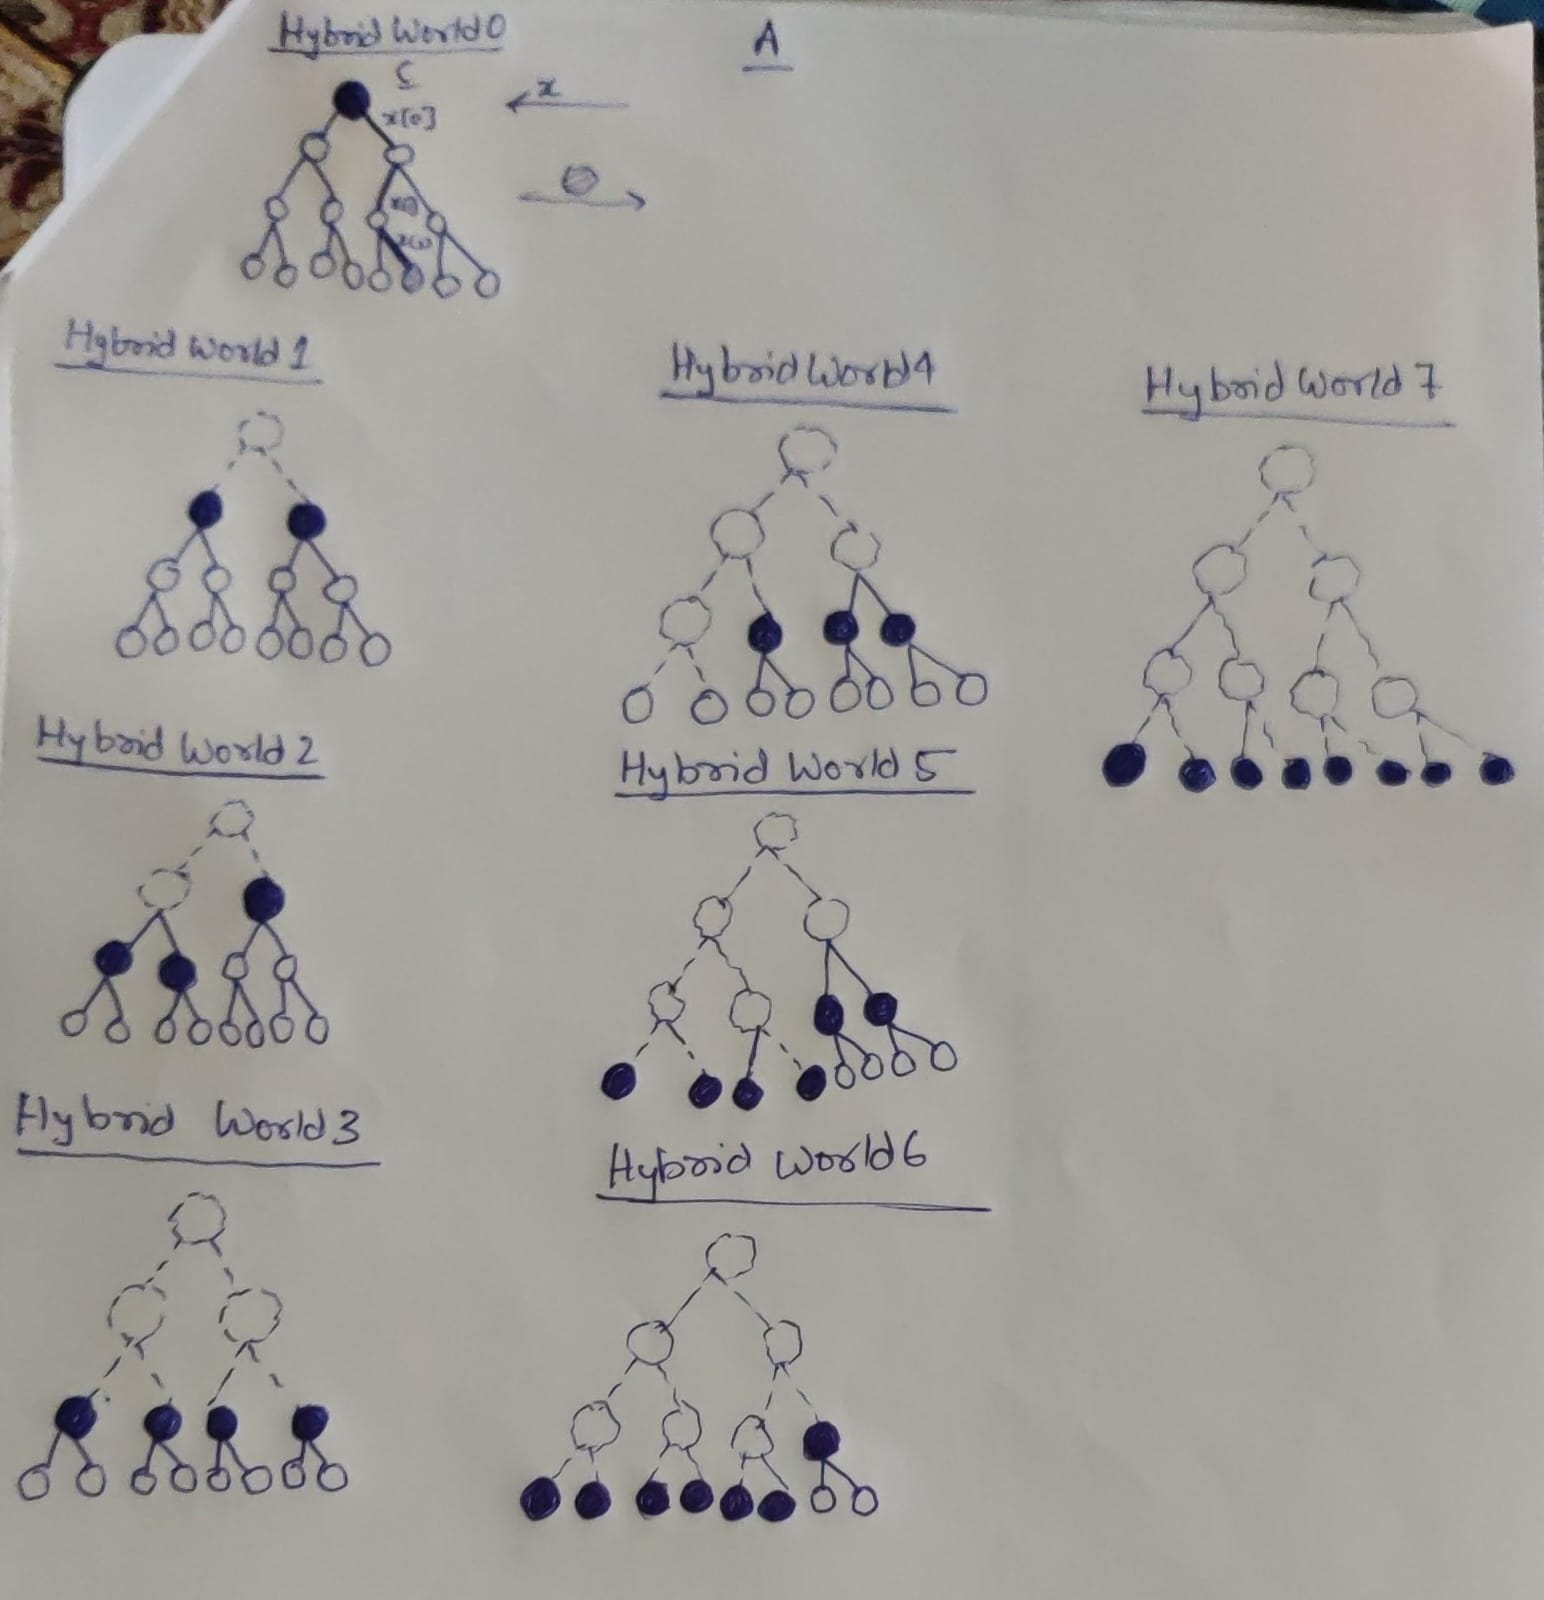
\includegraphics[scale=0.25]{images/Tree Construction.png}
        \caption{Construction of Hybrid worlds for the case $\log n=3$. The randomly generated nodes are shadedand the nodes which can be ignored are dotted}
        \label{fig:TC}
    \end{figure}
    \begin{enumerate}[(a)]
        \item  Construct $n$ hybrid worlds in the following way: In Hybrid $j$, the challenger builds an evaluation tree whose nodes are labeled as follows:
              \begin{itemize}
                  \item The first $j$ nodes (as appearing in the level order traversal of the tree) can be ignored.
                  \item The next $j + 1$ nodes are labelled with random values. 
                  \item Remaining nodes are derived from their parents.
              \end{itemize}
              In response to a query $x\in\bit^{\log n}$ in Hybrid $j$, the challenger sends to the adversary the label of the leaf addressed by $x$.

              Observe that Hybrid $0$ corresponds to the case $b=0$ in the PRF game when the challenger sends $F_k(x)$ and Hybrid $l$ corresponds to $b=1$ when the challenger uses a truly random function.

              \paragraph{Claim:} If there exists an adversary $\calA$ which can distinguish between Hybrid $i$ and Hybrid $i+1$ then we can construct an adversary $\calB$ which breaks the PRG security of $G$.

              \textit{Proof:} Consider the reduction \cref{red:p4a}

              \securitygame{Problem 4(a)}{Reduction for Problem 4(a)}{\label{red:p4a}}
              {
                  \begin{itemize}
                      \item Challenger picks a uniformly random bit $b \gets \bit$ and a seed $s\gets \bit^n$. If $b=0$, he sends $y=G(s)$ to $\calB$ otherwise he sends a $y=r\gets\bit^{2n}$.
                      \item $\calB$ constructs the evaluation tree. 
                      \begin{itemize}
                        \item The first $i+1$ nodes can be ignored
                        \item The next $i$ nodes are randomly generated
                        \item The next two nodes are made by splitting $y$ sent by the challenger into two halves
                        \item Remaining nodes are generated using the algorithm from their parents.
                      \end{itemize} 
                      \item The adversary $\calA$ makes polynomially many queries to $\calB$. In response to a query $x\in\bit^{\log n}$, $\calB$ sends the label of the leaf addressed by $x$ (This traveral is shown in the HybridWorld0 of \cref{red:p4a})
                      \item After polynomially many queries, $\calB$ forwards the response send by $\calA$ $(b')$ and wins if $b=b'$.
                  \end{itemize}
              }
              \begin{figure}[!ht]
                \centering
                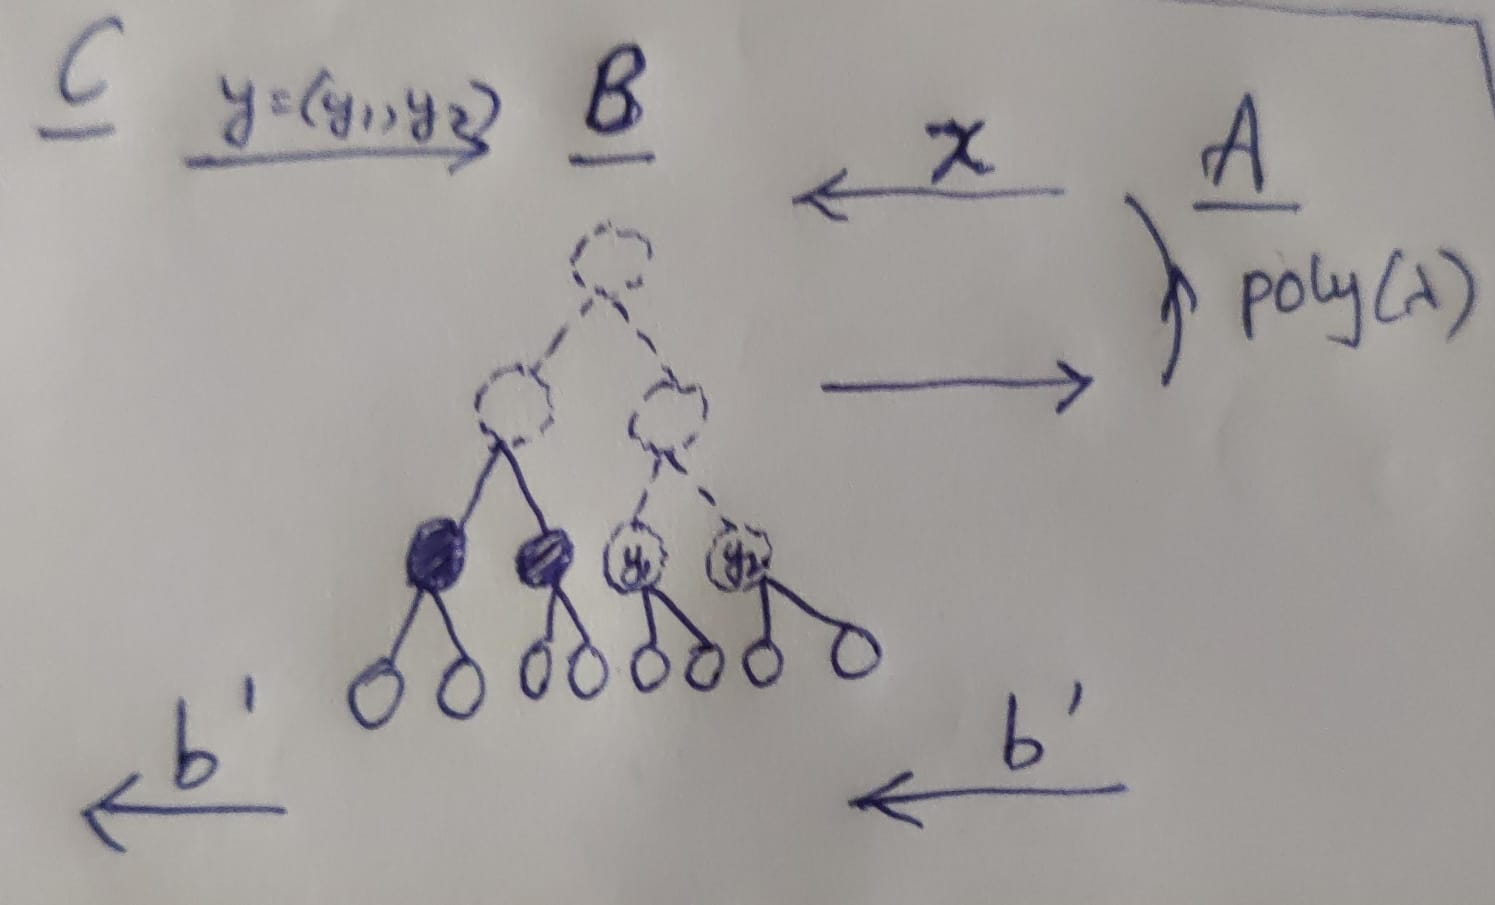
\includegraphics[scale=0.25]{images/Tree Red.png.jpg}
                \caption{Reduction for distinguishing between HybridWorld2 and HybridWorld3}
                \label{fig:p4a2}
              \end{figure}


                  From the construction, it can be checked that:
                  $$\Pr[b'=0|b=0]=\Pr[\calA\text{ outputs 0 in HybridWorld } i]=p_{i}$$
                  $$\Pr[b'=0|b=0]=\Pr[\calA\text{ outputs 0 in HybridWorld } i+1]=p_{i+1}$$
                  Thus,
                  $$\prg[\calB,\calG]=|p_{i}-p_{i+1}|$$
                  Finally for the combined reduction, we choose any one of the reductions at random.
                  $$\prg[\calB^c,\calG^c]=\frac{|p_{l}-p_{0}|}{n-1}$$
        \item In the above construction, $\calB$ will need to sample $O(2^d)$ random bitstrings in some hybrids, where $d$ is the depth of the tree. If $d=\log n$ then $\calB$ samples $O(n)$ bitstrings. However, if $d=n$ then he has to sample exponentially many strings, making him inefficient. So, we cannot use the same reduction when $x\in\bit^n$.
        \item The given construction is insecure. Consider an adversary $\calA$ which plays the following game $\calG$:
        \begin{itemize}
            \item $\calA$ sends $x$ to the Challenger and receives $y_1$
            \item $\calA$ sends $x||1$ to the Challenger and receives $y_2$
            \item $\calA$ finds $G(y_1)=(s_0,s_1)$ and checks if $s_1=y_1$. If so it returns $b'=0$ else $b'=1$
        \end{itemize}
        Now,
        $$\prf[\calA,\calG]=|\Pr[b'=0|b=0]-\Pr[b'=0|b=1]|$$
        From construction we have,
        $$\Pr[b'=0|b=0]=1$$
        and
        $$\Pr[b'=0|b=1]=\Pr[G(y_1)=(s_0,s_1)\wedge s_1=y_1]=2^{-n}$$
        Thus the $\prf[\calA,\calG]=1-2^{-n}$
        % \item The main problem in the above scheme occurs when one of the queries by the adversary is a proper prefix of the other. To avoid this, we modify the scheme by first applying a PRG on the query $x$. Let $\calG' = \{G'_n: \bit^n\rightarrow\bit^{l(n)}\}_{n\in\N}$ be a secure PRG family where $l(n)$ is poly-bounded. In the scheme, the challenger first applies $G'_n$ on the input $x$ sent by the adversary and then uses the tree construction replacing $x\mapsto G'_n(x)$.
        
        % The main intuition behind this construction is that for an \textit{efficient} adversary, it should be difficult to find $x_1,x_2, |x_1|=n_1<n_2=|x_2|$ such that $G'_{n_1}(x_1)$ is a proper prefix of $G'_{n_2}(x_2)$ (for example in the LWE construction). Then we can use Theorem 4.11 of the book which states that \textit{``If G is a secure PRG, then the variable length tree construction derived from G is a prefix-free secure PRF''}. So, this scheme is plausibly secure.
        \item The main problem in the above scheme occurs when one of the queries by the adversary is a proper prefix of the other. To avoid this, we modify the scheme by using $\calG = \{G_n: \bit^n\rightarrow\bit^{3n}\}_{n\in\N}$. Here, each node of the tree has 3 children. If a bit of $x$ is 0, we take the left most child. If it is 1, we take the central child and if x ends, we take the rightmost child. In this case, even if one of the queries is a prefix of the other, the adversary cannot distinguish if the challenger used the construction or a random bit (\cref{fig:modtree})
        \begin{figure}[!ht]
            \centering
            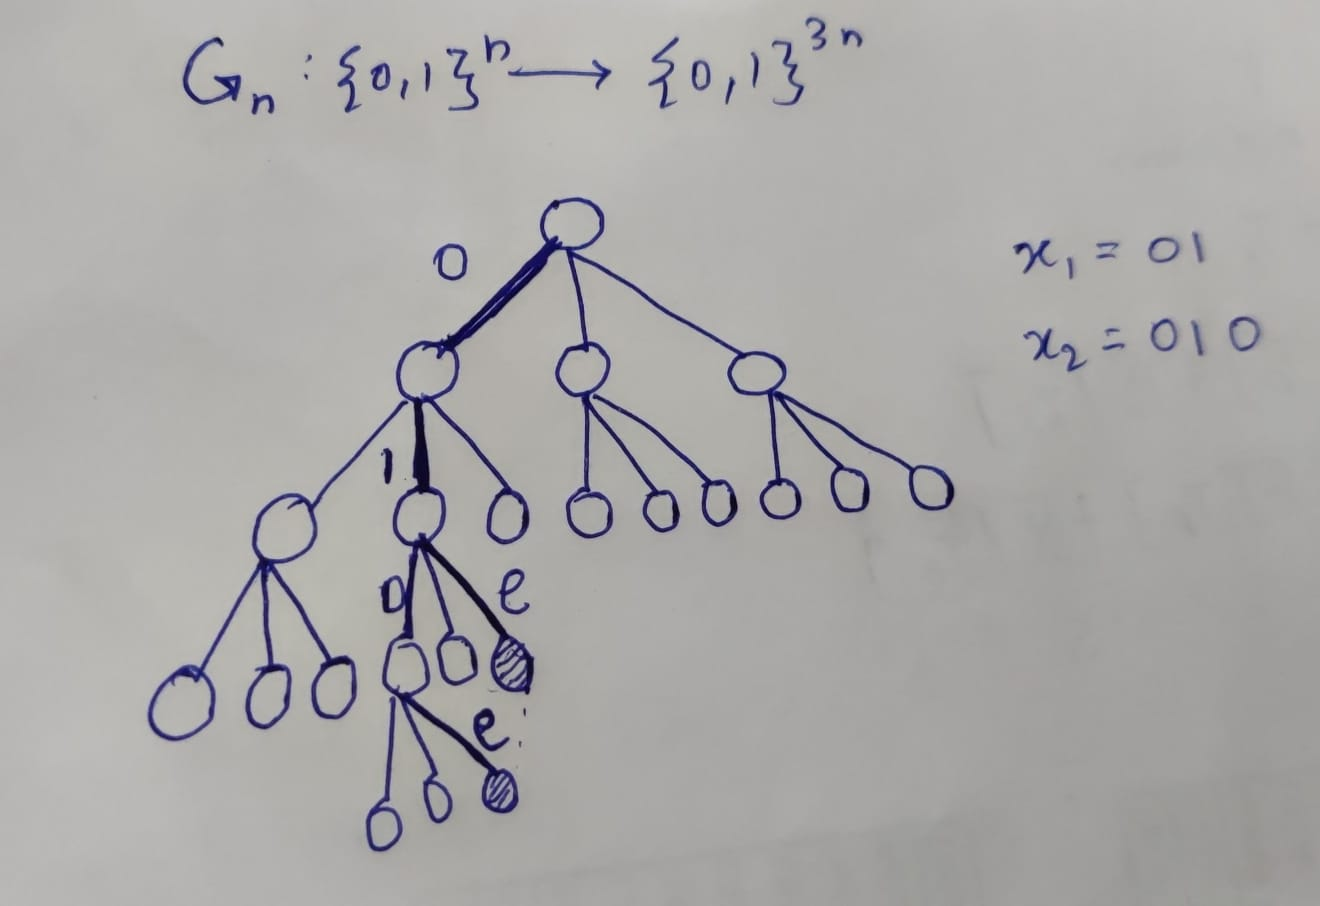
\includegraphics[scale=0.25]{images/Modified tree.jpg}
            \caption{The modified tree construction with $\calG = \{G_n: \bit^n\rightarrow\bit^{3n}\}_{n\in\N}$. Here the evaluation for $x_1=01$ and $x_2=010$ are shown. The shaded nodes are the outputs on the queries. As evident from the figure, the shaded nodes aren't directly related with each other. So, the adversary cannot break this scheme.}
            \label{fig:modtree}
        \end{figure}
    \end{enumerate}
\end{solution}


\prob{Part B : Coding Problems}
\begin{enumerate}
    \item \textbf{CRIME Attack: } The key observation for this attack is : 
    \begin{center} `` If \textsf{cmsg} contains a substring of the \textsf{cookie}, then the compressed string is shorter''\end{center}

     In our code, we attempt a brute-force attack on the encryption scheme by iteratively guessing and refining the secret cookie character by character, exploring alternative paths when multiple characters result in the same encrypted text length. The basic idea is to iteratively build the cookie by finding the character that, when appended to the current partial key, produces the shortest encrypted text. If multiple such characters exist, then they are all stored in a list and their alternative paths are explored too.

     \item \textbf{Attack on 2DES encryption: } Here, we implement a Meet-in-the-middle Attack on 2DES. Namely, we encrypt the messages using all possible keys and store them in a dictionary. We also decrypt the ciphertext using all possible keys and store them in a list. Finally, we search for the intermediary ciphertext by finding a common element in the dictionary and the list. The keys corresponding to this intermediary ciphertext are the keys we were searching for. Time complexity for the attack is $O(|\calK|)$
\end{enumerate}

\end{document}
